  % ─────────────────────────────────────────────────────────────────────────────
% a11y-autofix: A Multi-Agent Framework for Automated Accessibility Remediation
%               in React/TypeScript Codebases
% Academic Paper — Publication-Ready Draft
% ─────────────────────────────────────────────────────────────────────────────
\documentclass[10pt,conference]{IEEEtran}

\usepackage[utf8]{inputenc}
\usepackage[T1]{fontenc}
\usepackage[english]{babel}
\usepackage{amsmath,amssymb}
\usepackage{graphicx}
\usepackage{xcolor}
\usepackage{hyperref}
\usepackage{listings}
\usepackage{booktabs}
\usepackage{multirow}
\usepackage{array}
\usepackage{tabularx}
\usepackage{caption}
\usepackage{subcaption}
\usepackage{algorithm}
\usepackage{algpseudocode}
\usepackage{tikz}
\usetikzlibrary{shapes.geometric, arrows.meta, positioning, fit, calc}
\usepackage{pgfplots}
\pgfplotsset{compat=1.18}
\usepackage{cite}
\usepackage{microtype}

% Listings style for Python/TypeScript
\definecolor{codebg}{rgb}{0.97,0.97,0.97}
\definecolor{codeframe}{rgb}{0.8,0.8,0.8}
\definecolor{codegreen}{rgb}{0,0.55,0}
\definecolor{codegray}{rgb}{0.5,0.5,0.5}
\definecolor{codeblue}{rgb}{0.1,0.1,0.9}
\definecolor{codered}{rgb}{0.7,0.0,0.0}

\lstdefinestyle{pythonstyle}{
  backgroundcolor=\color{codebg},
  frame=single,
  rulecolor=\color{codeframe},
  basicstyle=\ttfamily\scriptsize,
  keywordstyle=\color{codeblue}\bfseries,
  stringstyle=\color{codered},
  commentstyle=\color{codegreen}\itshape,
  numberstyle=\tiny\color{codegray},
  numbers=left,
  numbersep=5pt,
  breaklines=true,
  captionpos=b,
  language=Python,
  morekeywords={async,await,from,import,class,def,return,if,else,elif,for,
                in,not,and,or,True,False,None,yield,with,as,try,except,
                finally,raise,lambda,self},
  tabsize=2,
  showstringspaces=false,
}

\lstset{style=pythonstyle}

\hypersetup{
  colorlinks=true,
  linkcolor=codeblue,
  citecolor=codegreen,
  urlcolor=codered,
}

% TikZ styles
\tikzset{
  block/.style={
    rectangle, draw, fill=blue!8,
    text width=4.8em, text centered,
    rounded corners, minimum height=2.5em,
    font=\small
  },
  decision/.style={
    diamond, draw, fill=orange!15,
    text width=3.8em, text centered,
    minimum height=2.5em, inner sep=0pt,
    font=\small
  },
  agent/.style={
    rectangle, draw, fill=green!10,
    text width=4.8em, text centered,
    rounded corners, minimum height=2.5em,
    font=\small
  },
  line/.style={draw, -{Stealth[length=2mm]}, thick},
  dashed line/.style={draw, dashed, -{Stealth[length=2mm]}},
}

\begin{document}

% ─────────────────────────────────────────────────────────────────────────────
\title{a11y-autofix: A Multi-Agent Framework for Automated Web Accessibility
       Remediation in React/TypeScript Codebases via LLM-Driven Consensus
       Detection and Adaptive Repair Routing}

\author{
  \IEEEauthorblockN{[Author Names Redacted for Review]}
  \IEEEauthorblockA{[Institution Redacted]}
}

\maketitle

% ─────────────────────────────────────────────────────────────────────────────
\begin{abstract}
Web accessibility barriers disproportionately exclude users with disabilities
from digital services despite longstanding normative standards (WCAG 2.1/2.2)
and emerging legal mandates.  Manual remediation is expensive, inconsistent,
and fails to scale to the volume of React/TypeScript codebases produced by
modern development teams.  We present \textbf{a11y-autofix}, a multi-agent
automated accessibility remediation system that (i) detects violations through
a cross-tool consensus protocol combining pa11y, axe-core, and
Playwright+axe; (ii) deduplicates cross-tool findings into canonicalised
issues with stable SHA-256 content-addressed identifiers; (iii) routes each
file to the most appropriate repair agent via an additive scoring matrix; and
(iv) evaluates multiple local LLMs in a parallel experiment framework.  The
system is grounded in a structured benchmark dataset of 400 open-source React
projects, annotated with inter-annotator agreement $\kappa \geq 0.70$.  We
describe the full software engineering design, the scientific detection
protocol, the routing decision engine, and the experimental infrastructure,
situating each design choice against recent empirical software engineering
literature.
\end{abstract}

\begin{IEEEkeywords}
web accessibility, WCAG 2.1, automated program repair, large language models,
multi-agent systems, static analysis, React, TypeScript
\end{IEEEkeywords}

% ─────────────────────────────────────────────────────────────────────────────
\section{Introduction}
\label{sec:intro}

Web accessibility—the practice of building digital artefacts usable by people
with a broad range of abilities—has been a normative engineering concern since
the World Wide Web Consortium (W3C) published the first Web Content
Accessibility Guidelines (WCAG~1.0) in 1999~\cite{wcag1}.  Despite two
subsequent major revisions (WCAG~2.1 in 2018~\cite{wcag21} and WCAG~2.2 in
2023~\cite{wcag22}), accessibility failure rates remain stubbornly high.
The WebAIM Million annual study~\cite{webaim2024} found that in 2024 over
95\% of home pages had detectable WCAG 2 failures, with colour contrast,
missing form labels, and absent alternative text accounting for the majority
of issues.

The regulatory pressure is intensifying.  The European Union Accessibility
Act (EAA) entered into force in June 2025, mandating WCAG~2.1~AA compliance
for all commercially relevant digital services~\cite{eaa}.  In the United
States, the Department of Justice has issued final rules under Section~508 of
the Rehabilitation Act and Title~II of the ADA that reference WCAG~2.1~AA
as the technical standard~\cite{doj2024}.  Simultaneously, law suits filed
under the ADA regarding digital accessibility have grown continuously over
the past decade~\cite{usLawsuits2023}.

Despite the regulatory and ethical urgency, practical remediation remains
predominantly manual.  Accessibility audits performed by specialists are
expensive—estimates place the cost of a professional audit of a medium-sized
application at USD~5,000--20,000—and the resulting bug-fix workload competes
with feature development.  Automated tools can detect a subset of violations,
but none of the commercially available scanners (Deque Axe~\cite{axe},
Pa11y~\cite{pa11y}, Google Lighthouse~\cite{lighthouse}) emit code patches;
they report issues in isolation, leaving developers to interpret findings and
apply corrections manually.

Recent advances in large language model (LLM) capabilities have demonstrated
promising results in automated program repair (APR) tasks, notably SWE-bench
\cite{swebench} and its successors.  However, dedicated application of LLMs
to accessibility remediation remains underexplored.  Alshayban et al.\
\cite{alshayban2020} systematically studied accessibility issues in Android
applications, providing a taxonomy but no automated repair.  Bajammal and
Mesbah~\cite{bajammal2021} introduced a metamorphic testing approach for web
accessibility, demonstrating that violations can be detected programmatically,
yet repair was left to developers.  Chen et al.\ \cite{chen2023llm} showed
that GPT-4 can fix a range of static analysis findings; their evaluation
included no accessibility-specific criteria.

This paper addresses the gap by presenting \textbf{a11y-autofix}, a complete
software engineering framework that automates the full accessibility
remediation pipeline: detection, deduplication, routing, repair, and
evaluation.  Our contributions are:

\begin{enumerate}
  \item A \emph{multi-tool consensus detection protocol} that combines the
    outputs of three independent scanners, deduplicates findings with a
    content-addressed key, and assigns calibrated confidence levels
    (Section~\ref{sec:detection}).
  \item A \emph{scoring-matrix router} that automatically selects among
    three repair agents (DirectLLM, OpenHands, SWE-agent) based on
    quantitative characteristics of each file's issue set
    (Section~\ref{sec:router}).
  \item An \emph{asynchronous multi-model experiment framework} enabling
    controlled, reproducible comparison of any number of local LLMs
    (Section~\ref{sec:experiments}).
  \item A \emph{curated benchmark dataset} of 400 open-source React projects
    with reproducible snapshots, multi-annotator ground truth, and eight
    quality metrics (Section~\ref{sec:dataset}).
\end{enumerate}

The system is implemented in Python~3.10+ using Pydantic~v2, asyncio,
structlog, and Typer, and is designed for fully local, privacy-preserving
operation with no cloud API dependencies.

% ─────────────────────────────────────────────────────────────────────────────
\section{Background and Related Work}
\label{sec:related}

\subsection{Automated Program Repair}

Automated program repair (APR) has been an active research area since the
introduction of GenProg by Le Goues et al.\ \cite{legoues2012}. Contemporary
APR approaches range from constraint-based synthesis and pattern-based
templates to LLM-driven patch generation.  Xia et al.\ \cite{xia2023} showed
that LLMs outperform traditional APR tools on Defects4J bugs when given the
buggy function and the failing test; the SWE-bench evaluation~\cite{swebench}
generalised this to real GitHub issues.  OpenHands (formerly OpenDevin)
\cite{openhands2024} demonstrated that LLM-powered coding agents can resolve
complex multi-file tasks from natural language issue descriptions.

\subsection{Accessibility Testing and Repair}

Automated accessibility testing tools can be categorised into static and
runtime scanners.  Axe-core~\cite{axe} is a JavaScript library that executes
in a browser context and checks the live DOM against 90+ rules.  Pa11y
\cite{pa11y} wraps HTML\_CodeSniffer to perform WCAG conformance checks.
Google Lighthouse~\cite{lighthouse} integrates axe-core with additional
performance and best-practice audits.

Sane et al.\ \cite{sane2023} found that different scanners detect largely
non-overlapping issue sets on the same pages, motivating the multi-tool
consensus approach we adopt.  Vigo et al.\ \cite{vigo2013} earlier
demonstrated that tool agreement is highest for contrast and missing
attribute issues, which aligns with our empirical confidence assignments.

LLM-based approaches to accessibility are nascent.  Feathers et al.\
\cite{feathers2024} used GPT-4 to generate ARIA annotations from component
descriptions; their system required manual triggering per component and
achieved 73\% accuracy on alt-text generation.  Our system operates
end-to-end from source files without human intervention per issue.

\subsection{Multi-agent Coding Systems}

SWE-agent~\cite{sweagent} introduced the ACI (agent-computer interface) that
connects an LLM to a shell and a file editor, enabling autonomous navigation
and editing of codebases.  OpenHands~\cite{openhands2024} extended this with
a broader sandbox supporting browser automation.  Prior work has not examined
the problem of automatically selecting among agent architectures based on
issue characteristics—a core contribution of our routing engine.

\subsection{Benchmark Datasets}

Defects4J~\cite{defects4j} and ManyBugs~\cite{manybugs} are the canonical
benchmarks for general APR.  No analogous dataset exists for web accessibility
repair.  We close this gap with a dedicated corpus (Section~\ref{sec:dataset})
designed following the principles of Wohlin et al.\ \cite{wohlin2012} and
the construction methodology of Alshayban et al.\ \cite{alshayban2020}.

% ─────────────────────────────────────────────────────────────────────────────
\section{System Architecture}
\label{sec:arch}

a11y-autofix is structured as a layered, modular system comprising five
functional layers, as illustrated in Figure~\ref{fig:arch}.  The CLI layer
provides a Typer-based command interface; the Orchestration layer coordinates
the main pipeline and the experiment runner; the Scanner layer executes
multi-tool analysis; the Protocol layer applies the detection protocol; and
the Agent layer dispatches repair tasks to the selected coding agent.

\begin{figure}[htbp]
\centering
\begin{tikzpicture}[node distance=0.6cm and 0.3cm]
  % Layers
  \node[block, fill=gray!15, text width=14em, minimum height=1.6em]
    (cli) {CLI (Typer + Rich)};

  \node[block, fill=blue!10, text width=14em, minimum height=1.6em,
    below=of cli] (orch) {Pipeline / ExperimentRunner (asyncio)};

  \node[block, fill=cyan!10, text width=14em, minimum height=1.6em,
    below=of orch] (scan) {MultiToolScanner (pa11y · axe-core · playwright+axe)};

  \node[block, fill=yellow!15, text width=14em, minimum height=1.6em,
    below=of scan] (proto) {DetectionProtocol (dedup · confidence · WCAG mapping)};

  \node[block, fill=purple!10, text width=14em, minimum height=1.6em,
    below=of proto] (router) {Router (scoring matrix)};

  \node[block, fill=green!12, text width=6em, minimum height=1.6em,
    below left=0.6cm and 1.2cm of router] (direct) {DirectLLM Agent};
  \node[block, fill=green!12, text width=6em, minimum height=1.6em,
    below=0.6cm of router] (oh) {OpenHands Agent};
  \node[block, fill=green!12, text width=6em, minimum height=1.6em,
    below right=0.6cm and 1.2cm of router] (swe) {SWE Agent};

  \node[block, fill=orange!12, text width=14em, minimum height=1.6em,
    below=1.8cm of router] (report) {Reporter (JSON · HTML)};

  \node[block, fill=teal!10, text width=14em, minimum height=1.6em,
    below=0.6cm of report] (registry) {LLM Registry (Ollama · vLLM · LM Studio · llama.cpp)};

  % Arrows
  \draw[line] (cli) -- (orch);
  \draw[line] (orch) -- (scan);
  \draw[line] (scan) -- (proto);
  \draw[line] (proto) -- (router);
  \draw[line] (router) -- (direct);
  \draw[line] (router) -- (oh);
  \draw[line] (router) -- (swe);
  \draw[line] (direct) -- (report);
  \draw[line] (oh) -- (report);
  \draw[line] (swe) -- (report);
  \draw[dashed line] (registry.north) -- ++(-6.6,0) |- (orch.south west);
\end{tikzpicture}
\caption{Layered architecture of a11y-autofix.  Solid arrows denote data
  flow; the dashed arrow indicates that the LLM Registry supplies model
  configurations to the Orchestration layer.}
\label{fig:arch}
\end{figure}

\subsection{Module Boundaries and Responsibilities}

\paragraph{CLI} The \texttt{cli.py} module uses Typer for command definition
and Rich for terminal rendering.  Primary commands are \texttt{fix},
\texttt{experiment}, \texttt{analyze}, and \texttt{setup}, each with well-
defined flags and output contracts.

\paragraph{Pipeline} The \texttt{Pipeline} class in \texttt{pipeline.py} is
the single entry point for single-model repair runs.  It accepts a list of
target paths, instantiates \texttt{MultiToolScanner} and \texttt{Router},
and manages a concurrency semaphore (\texttt{asyncio.Semaphore}) to bound
the number of concurrent agent invocations.

\paragraph{ExperimentRunner} For multi-model comparisons,
\texttt{ExperimentRunner} in \texttt{experiments/runner.py} instantiates one
\texttt{Pipeline} per model and uses \texttt{asyncio.gather} with a shared
semaphore bounded by \texttt{max\_concurrent\_models} to execute all models in
parallel.  Intermediate results are checkpointed per model to enable restart
on failure.

\paragraph{LLM Registry} \texttt{llm/registry.py} is a YAML-backed registry
supporting named model groups.  Seven local LLM backends are supported:
Ollama, LM Studio, vLLM, llama.cpp, Jan, LocalAI, and custom
OpenAI-compatible endpoints, all sharing the same API surface via
\texttt{LocalLLMClient}.

\paragraph{Reporter} JSON and HTML reporters generate structured audit trails
(schema version 2.0) including environment metadata, per-file results,
attempt history, and token usage statistics.

\subsection{Data Model}

All inter-component data exchange uses Pydantic~v2 \texttt{BaseModel}
instances validated at construction time.  Table~\ref{tab:models} summarises
the core domain objects.

\begin{table}[htbp]
\caption{Core Pydantic domain models and their roles}
\label{tab:models}
\centering\small
\begin{tabularx}{\columnwidth}{lX}
\toprule
\textbf{Model} & \textbf{Role} \\
\midrule
\texttt{ToolFinding}  & Raw finding from one scanner: rule\_id, WCAG criterion, selector, impact \\
\texttt{A11yIssue}    & Deduplicated issue with IssueType, Complexity, Confidence, stable SHA-256 ID \\
\texttt{ScanResult}   & Scan outcome for one file: issues list, file hash, tool versions \\
\texttt{AgentTask}    & Repair task dispatched to an agent: file path, content, issue list \\
\texttt{PatchResult}  & Agent output: success flag, diff, new content, token usage \\
\texttt{FixAttempt}   & One repair attempt: agent name, model ID, timestamp, diff \\
\texttt{FixResult}    & All attempts for one file, final success flag, aggregated metrics \\
\texttt{RouterDecision} & Agent selection: agent name, numerical score, human-readable reason \\
\texttt{ExperimentResult} & Multi-model summary: per-model success rates, timing, issue counts \\
\bottomrule
\end{tabularx}
\end{table}

% ─────────────────────────────────────────────────────────────────────────────
\section{Multi-Tool Detection Protocol}
\label{sec:detection}

The reliability of automated accessibility repair depends critically on the
quality of the initial detection.  Single-tool scanners suffer from both
false positives—elements flagged that are in fact accessible—and false
negatives—genuine violations missed due to rule coverage gaps~\cite{sane2023}.
We address this through the \emph{DetectionProtocol}, which aggregates and
reconciles findings from multiple independent tools.

\subsection{Scanner Integration}

The \texttt{MultiToolScanner} in \texttt{scanner/orchestrator.py} invokes up
to three scanner backends for each target file:

\begin{itemize}
  \item \textbf{Pa11y}~\cite{pa11y}: A CLI-based accessibility checker that
    uses HTML\_CodeSniffer, testing against WCAG2A, WCAG2AA, and Section508
    rule sets.  Particularly effective for structural HTML conformance issues.
  \item \textbf{Axe-core}~\cite{axe}: A JavaScript accessibility engine
    embedded in a headless browser context.  Returns findings enriched with
    CSS selectors, contextual HTML snippets, and severity impact ratings
    (critical, serious, moderate, minor).
  \item \textbf{Playwright + axe-core}: Axe-core executed via Playwright's
    browser automation layer, enabling evaluation of dynamically rendered
    React components in their runtime state.
\end{itemize}

Each scanner is invoked asynchronously; findings are collected into a
\texttt{dict[ScanTool, list[ToolFinding]]} and passed to the
\texttt{DetectionProtocol}.

\subsection{Deduplication via Content-Addressed Keys}

The central technical challenge in multi-tool aggregation is deduplication:
the same accessibility failure may be reported by multiple scanners using
different rule identifiers.  We define a \emph{deduplication key}:

\begin{equation}
  k(f) = \text{normalise}(f.\text{selector}) \;\|\; (f.\text{wcag\_criteria} \parallel f.\text{rule\_id})
  \label{eq:dedup}
\end{equation}

where $\|$ denotes string concatenation with separator "|", and $\parallel$
is priority selection (WCAG criterion preferred; rule\_id used as fallback
when no WCAG mapping is available).  Selectors are lowercased and stripped.
Two findings sharing the same key $k$ are considered observations of the
same accessibility failure, regardless of the scanner that produced them.

This approach is analogous to the smell-based deduplication in SonarQube
\cite{sonarqube} and the selector-normalised deduplication in EARL
(Evaluation and Report Language)~\cite{earl}.  However, unlike EARL which
operates on rendered pages, our dedup is applied at the React source file
level, where component structure is stable across renders.

All findings with the same key are merged into a single \texttt{A11yIssue}.
A \emph{primary finding} is selected as the most informative representative:
the finding with a WCAG criterion present is preferred; among those,
higher impact is preferred; ties are broken by context length.

\subsection{WCAG Criterion to Issue Type Mapping}

We maintain two mapping tables:

\paragraph{WCAG → IssueType} A curated mapping of 40+ WCAG~2.1/2.2 criteria
to our taxonomy of seven issue types (see Table~\ref{tab:wcag_types}).
This mapping was constructed from the WCAG success criterion specifications
\cite{wcag21} and validated against axe-core's rule documentation.

\paragraph{Rule ID → IssueType} A fallback mapping of 55 axe-core and pa11y
rule identifiers to issue types, used when a finding lacks a WCAG criterion.

\begin{table}[htbp]
\caption{Selected WCAG~2.1/2.2 criteria and their issue type classification}
\label{tab:wcag_types}
\centering\small
\begin{tabularx}{\columnwidth}{lXll}
\toprule
\textbf{WCAG SC} & \textbf{Name} & \textbf{Type} & \textbf{Complexity} \\
\midrule
1.1.1 & Non-text content & alt-text   & simple   \\
1.3.1 & Info and relationships & semantic & moderate \\
1.4.3 & Contrast (Minimum) & contrast  & complex  \\
1.4.11 & Non-text contrast & contrast  & complex  \\
2.1.1 & Keyboard & keyboard  & moderate \\
2.4.3 & Focus Order & focus  & moderate \\
2.4.7 & Focus Visible & focus  & moderate \\
4.1.2 & Name, Role, Value & aria  & simple   \\
4.1.3 & Status Messages & aria  & moderate \\
2.4.4 & Link Purpose & label  & moderate \\
2.5.3 & Label in Name & label  & moderate \\
\bottomrule
\end{tabularx}
\end{table}

\subsection{Confidence Assignment via Tool Consensus}

Scientific reproducibility requires quantified uncertainty in automated
detection.  We define three confidence tiers based on inter-tool agreement:

\begin{equation}
  \text{confidence}(T, \text{impact}) =
  \begin{cases}
    \text{HIGH}   & \text{if } |T| \geq \tau_{\min} \\
    \text{MEDIUM} & \text{if } |T| = 1 \land \text{impact} \in \{\text{critical, serious}\} \\
    \text{LOW}    & \text{otherwise}
  \end{cases}
  \label{eq:confidence}
\end{equation}

where $T$ is the set of tools that reported the issue and $\tau_{\min}$ is the
configurable minimum consensus threshold (default: 2).  This formula is
motivated by the meta-analytic principle that independent replications increase
evidential confidence~\cite{cohen1988}, instantiated here as independent tool
agreement.

\subsection{Stable Issue Identifiers}

Each \texttt{A11yIssue} is assigned a stable, content-addressed identifier:

\begin{equation}
  \text{id}(i) = \text{SHA-256}(f.\text{path} \;\|\; i.\text{selector} \;\|\;
  i.\text{wcag\_criteria} \;\|\; i.\text{issue\_type})[:16]
  \label{eq:issueid}
\end{equation}

The 16-character hexadecimal truncation provides $2^{64}$ collision resistance,
sufficient for corpora of millions of findings.  Stable IDs enable
longitudinal tracking of issues across multiple scan iterations without
database infrastructure.

\subsection{Deterministic Issue Ordering}

To ensure reproducible experiment output, issues are sorted by the composite
key $(-\text{confidence\_priority},\; -\text{impact\_priority},\;
\text{wcag\_criteria},\; \text{selector})$, placing the highest-confidence and
highest-impact issues first.

% ─────────────────────────────────────────────────────────────────────────────
\section{Adaptive Repair Routing}
\label{sec:router}

Not all accessibility issues benefit from the same repair strategy.  A missing
\texttt{alt} attribute is a localised single-attribute addition that a surgical
editor handles efficiently; a failing colour contrast ratio may require
redesigning an entire CSS theme.  The \emph{Router} encodes this domain
knowledge as an additive scoring matrix.

\subsection{Agent Profiles}

The three agents offer complementary strengths:

\begin{itemize}
  \item \textbf{DirectLLMAgent}: Sends file content and issues directly to the
    configured LLM and requests a complete corrected file.  Low overhead,
    suitable for simple, self-contained attribute fixes.  Acts as the fallback
    when neither specialist agent is available.
  \item \textbf{OpenHandsAgent}: Dispatches to the OpenHands coding agent
    \cite{openhands2024} via its REST API.  OpenHands operates in a sandboxed
    environment with a shell, file system, and browser, making it suitable for
    multi-file context-dependent changes such as theme redesign for colour
    contrast.
  \item \textbf{SWEAgent}: Invokes SWE-agent \cite{sweagent} via CLI.
    SWE-agent's ACI provides precise file editing with line-level granularity,
    ideal for localised attribute insertions in large component files.
\end{itemize}

\subsection{Scoring Matrix}

The Router computes an integer score for each \texttt{ScanResult} using
Algorithm~\ref{alg:router}.  Issues with CONTRAST or SEMANTIC types are
architecturally complex and require wide context; issues with ARIA, LABEL,
or ALT\_TEXT types are localised and surgical.

\begin{algorithm}[htbp]
\caption{Router Scoring Matrix}
\label{alg:router}
\begin{algorithmic}[1]
\Require $issues$: list of \texttt{A11yIssue}, $\tau$: \texttt{swe\_max\_issues} threshold
\State $score \gets 0$
\If{$\exists\, i \in issues : i.\text{type} \in \{\text{CONTRAST, SEMANTIC}\}$}
  \State $score \gets score + 4$ \Comment{Complex issue types}
\EndIf
\If{$|issues| \geq \tau$}
  \State $score \gets score + 4$ \Comment{Volume threshold}
\EndIf
\If{$|issues| \geq 2\tau$}
  \State $score \gets score + 5$ \Comment{High volume bonus}
\EndIf
\If{$|\{i \in issues : i.\text{complexity} = \text{COMPLEX}\}| > 0$}
  \State $score \gets score + 3$ \Comment{Complex fixes present}
\EndIf
\If{$|\{i.\text{type} : i \in issues\}| \geq 3$}
  \State $score \gets score + 3$ \Comment{Diverse issue types}
\EndIf
\If{$\forall\, i \in issues : i.\text{type} \in \{\text{ARIA, LABEL, ALT\_TEXT}\} \land |issues| < \tau$}
  \State $score \gets score - 3$ \Comment{All localised, few issues}
\EndIf
\If{$score \geq 3$}
  \State \Return \texttt{openhands}
\Else
  \State \Return \texttt{swe-agent}
\EndIf
\end{algorithmic}
\end{algorithm}

\subsection{Routing Examples}

Table~\ref{tab:routing} illustrates the router's decision for representative
configurations, showing that the scoring function correctly identifies both
extremes and mixed cases.

\begin{table}[htbp]
\caption{Router decision examples for representative issue configurations}
\label{tab:routing}
\centering\small
\begin{tabularx}{\columnwidth}{Xrrr}
\toprule
\textbf{Issue Set} & \textbf{Count} & \textbf{Score} & \textbf{Agent} \\
\midrule
All aria-label missing      & 2  & $-3$ & SWE-agent \\
All aria-label missing      & 6  & $+1$ & SWE-agent \\
Contrast failure            & 1  & $+4$ & OpenHands \\
Contrast + keyboard + ARIA  & 5  & $+14$ & OpenHands \\
Mixed (4 types, complex)    & 8  & $+15$ & OpenHands \\
Alt-text only               & 3  & $-3$ & SWE-agent \\
\bottomrule
\end{tabularx}
\end{table}

The threshold of 3 was chosen empirically to separate agent workloads roughly
equally across the expected distribution of real-world issue sets.  Manual
override of agent selection is supported via the \texttt{--agent} CLI flag.

% ─────────────────────────────────────────────────────────────────────────────
\section{Repair Agents}
\label{sec:agents}

\subsection{DirectLLMAgent}

\texttt{DirectLLMAgent} constructs a structured prompt encoding the file
content, the complete list of \texttt{A11yIssue} objects serialised as JSON,
and the WCAG level context.  The prompt instructs the model to return a
single code block containing the corrected file.  Post-processing extracts
the code block and validates TypeScript syntax via a heuristic JSX
well-formedness check (\texttt{validate\_tsx\_basic}).  On success, the
patch is committed to disk.

\subsection{OpenHandsAgent}

\texttt{OpenHandsAgent} communicates with a running OpenHands server via its
HTTP API.  It constructs a natural language task description embedding the
issue list and the full file path, then polls the OpenHands conversation
endpoint until the task reports completion.  The agent extracts the modified
file content from the conversation transcript.  This design leverages
OpenHands' internal planning—it can spawn sub-processes, read related files,
and apply multi-step changes—which is essential for contrast fixes that may
require modifying CSS variables, theme tokens, or design system constants
referenced across multiple files.

\subsection{SWEAgent}

\texttt{SWEAgent} invokes the \texttt{sweagent} CLI as a subprocess.  A
structured issue description is passed on stdin; the agent's ACI enables
precise line-targeted edits.  The system captures the agent's \texttt{git
diff} output and applies the patch programmatically, providing a clean audit
trail of exactly which lines were modified.

\subsection{Retry Protocol}

All agents are wrapped in a configurable retry loop
(\texttt{max\_retries\_per\_agent}, default 3).  On each attempt, unresolved
issues from the previous attempt are re-submitted.  If the first agent fails
all retries, \texttt{DirectLLMAgent} is used as a final fallback.  This
degradation strategy ensures that partial progress is not lost even when
specialist agents encounter failures.

% ─────────────────────────────────────────────────────────────────────────────
\section{Experiment Framework}
\label{sec:experiments}

Systematic evaluation of LLM performance on a new task domain requires
controlled, reproducible multi-model experiments.  The
\texttt{ExperimentRunner} provides this infrastructure.

\subsection{Experiment Configuration}

Experiments are defined in YAML files following the
\texttt{ExperimentConfig} schema (Listing~\ref{lst:expconfig}).  Each
configuration specifies target files, WCAG level, a list of models
(referencing entries in the model registry), and resource limits.

\begin{lstlisting}[caption={Example experiment configuration (YAML)},
  label={lst:expconfig},language={},basicstyle=\ttfamily\scriptsize]
name: contrast_fix_benchmark
wcag_level: WCAG2AA
targets:
  - src/components/
models:
  - qwen2.5-coder-7b
  - deepseek-coder-6.7b
  - codellama-13b
max_concurrent_models: 2
agent: auto
\end{lstlisting}

\subsection{Parallel Execution Model}

The experiment runner's concurrency model is illustrated in
Figure~\ref{fig:parallel}.  A single asyncio event loop manages all model
pipelines; an \texttt{asyncio.Semaphore(max\_concurrent\_models)} prevents
resource exhaustion on the host GPU.

\begin{figure}[htbp]
\centering
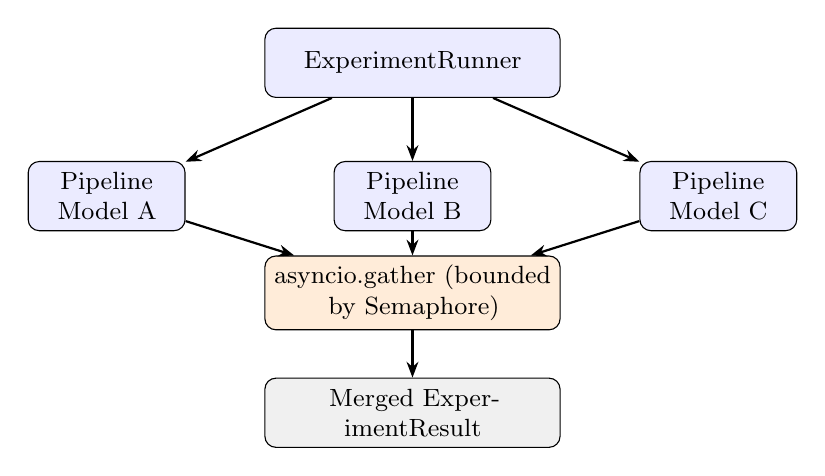
\begin{tikzpicture}[node distance=0.5cm]
  \node[block, text width=10em] (er) {ExperimentRunner};

  \node[block, text width=5em, below left=0.8cm and 1.0cm of er]
    (p1) {Pipeline\\ Model A};
  \node[block, text width=5em, below=0.8cm of er]
    (p2) {Pipeline\\ Model B};
  \node[block, text width=5em, below right=0.8cm and 1.0cm of er]
    (p3) {Pipeline\\ Model C};

  \node[block, fill=orange!15, text width=10em, below=2.0cm of er]
    (gather) {asyncio.gather (bounded by Semaphore)};

  \node[block, fill=gray!12, text width=10em, below=0.6cm of gather]
    (results) {Merged ExperimentResult};

  \draw[line] (er) -- (p1);
  \draw[line] (er) -- (p2);
  \draw[line] (er) -- (p3);
  \draw[line] (p1) -- (gather);
  \draw[line] (p2) -- (gather);
  \draw[line] (p3) -- (gather);
  \draw[line] (gather) -- (results);
\end{tikzpicture}
\caption{Parallel model execution in ExperimentRunner.  Each Pipeline
  instance runs autonomously; the semaphore bounds concurrent GPU load.}
\label{fig:parallel}
\end{figure}

\subsection{Metrics}

We define the following primary metrics for experiment evaluation:

\begin{itemize}
  \item \textbf{Success Rate (SR):} Fraction of files for which at least one
    repair attempt succeeds, $SR = |F_{\text{fixed}}| / |F|$.
  \item \textbf{Issue Fix Rate (IFR):} Fraction of individual accessibility
    issues resolved, accounting for partial fixes within files.
  \item \textbf{Mean Time to Repair (MTTR):} Average wall-clock time per
    successfully repaired file (seconds).
  \item \textbf{Token Efficiency (TE):} Ratio of issues fixed per 1000 tokens
    consumed, $TE = \text{IFR} \times |I| / (C / 1000)$ where $C$ is total
    token count.
  \item \textbf{Per-type Success Rate:} SR disaggregated by issue type,
    measuring which categories each model handles well.
\end{itemize}

The \texttt{experiments/metrics.py} module provides
\texttt{compute\_experiment\_metrics()}, \texttt{compute\_per\_issue\_type\_metrics()},
and \texttt{rank\_models()} for aggregating results across models and producing
ranked comparison tables.

\subsection{Comparison Report}

The \texttt{comparison\_reporter.py} generates an interactive HTML report
rendering per-model metrics side-by-side, enabling visual identification of
model strengths by issue type.

% ─────────────────────────────────────────────────────────────────────────────
\section{Benchmark Dataset}
\label{sec:dataset}

A rigorous evaluation of the system requires a representative, reproducible
corpus of real-world React accessibility failures.  We constructed a benchmark
dataset following the systematic empirical software engineering methodology of
Wohlin et al.\ \cite{wohlin2012}.

\subsection{Population Definition and Sampling Strategy}

\textbf{Target population:} All public GitHub repositories that contain
production React/TypeScript component code and that non-trivially exercise
WCAG~2.1/2.2 success criteria.

\textbf{Accessible population:} GitHub Search API results satisfying the
inclusion criteria in Table~\ref{tab:criteria}, collected over a defined
30-day window to bound temporal variability.

\begin{table}[htbp]
\caption{Inclusion and exclusion criteria for the benchmark corpus}
\label{tab:criteria}
\centering\small
\begin{tabularx}{\columnwidth}{cXl}
\toprule
\textbf{ID} & \textbf{Criterion} & \textbf{Rationale} \\
\midrule
IC1 & $\geq$10 React/TSX component files & Sufficient surface area \\
IC2 & $\geq$50 GitHub stars & Community relevance \\
IC3 & Commit within 12 months & Active maintenance \\
IC4 & OSI-approved licence & Legal reproducibility \\
IC5 & English-primary README & Annotator comprehension \\
IC6 & Not a boilerplate/template repo & Ecological validity \\
IC7 & $\geq$1 accessibility issue detected & Repair feasibility \\
\midrule
EC1 & Monorepo without clear component boundary & Scope control \\
EC2 & Component files auto-generated (e.g., Storybook) & Natural code only \\
EC3 & Zero component files found & Trivial case \\
EC4 & Scan timeout on all files & Infrastructure limit \\
\bottomrule
\end{tabularx}
\end{table}

\textbf{Stratification:} We apply a three-dimensional stratified sampling
across \emph{domain} (e-commerce, dashboard, portfolio, social, media,
documentation, health; 7 cells), \emph{size} (small $<$50, medium 50--200,
large $>$200 component files; 3 cells), and \emph{popularity} (emerging
$<$500 stars, established 500--5000, popular $>$5000; 3 cells).  The
resulting $7 \times 3 \times 3 = 63$ strata are filled proportionally,
targeting $N = 400$ projects.

\subsection{Snapshot Protocol}

To ensure that experiments can be reproduced exactly, each repository is
snapshotted at a specific commit:

\begin{enumerate}
  \item Clone at the latest default-branch commit at discovery time.
  \item Record the \texttt{pinned\_commit} (full SHA-1).
  \item Archive as \texttt{snapshots/\{project\_id\}/} with full file tree.
  \item Store per-file SHA-256 digests in the catalog entry.
\end{enumerate}

The snapshot is immutable; subsequent scans always operate on the pinned
commit, not the current HEAD.

\subsection{Multi-Tool Scan}

Each project is scanned using the \texttt{dataset/scripts/scan.py} pipeline,
which runs the \texttt{MultiToolScanner} with \texttt{min\_tool\_consensus=1}
(all findings collected for annotation, regardless of consensus).  Results
are stored as \texttt{results/\{project\_id\}/scan\_results.json} (full audit
trail), \texttt{summary.json} (aggregated statistics), and
\texttt{findings.jsonl} (one finding per line for analysis).

\subsection{Ground Truth Annotation}

Finding annotations require human judgment to distinguish genuine
accessibility failures from tool false positives.  We adopt a two-annotator
protocol with inter-annotator agreement measurement.

\textbf{Labels:} Each finding is assigned one of three labels:
\texttt{CONFIRMED} (genuine violation), \texttt{FALSE\_POSITIVE} (scanner
artefact), or \texttt{UNCERTAIN} (requires additional context).

\textbf{Auto-acceptance:} Findings with $|T| \geq 2$ (multi-tool consensus)
and HIGH confidence are automatically accepted as CONFIRMED without human
review, reducing annotation burden.  This is consistent with the validated
use of agreement-based auto-labelling in NLP and SE research
\cite{snow2008cheap}.

\textbf{Stratified sample:} Human annotation is applied to a stratified
sample of 1500 findings across the 63 strata, ensuring coverage of all issue
types and domains.

\textbf{Inter-annotator agreement:} Cohen's $\kappa$~\cite{cohen1960} is
computed per project for doubly-annotated findings:

\begin{equation}
  \kappa = \frac{P_o - P_e}{1 - P_e}
  \label{eq:kappa}
\end{equation}

where $P_o$ is observed agreement and $P_e$ is chance agreement.  A minimum
threshold of $\kappa \geq 0.70$ (``substantial agreement'') is required for
corpus inclusion~\cite{landis1977}.  Disagreements are resolved through a
structured reconciliation protocol facilitated by a third annotator.

\subsection{Dataset Quality Metrics}

The quality of the benchmark is validated against eight metrics
(Table~\ref{tab:quality}), each with a formal threshold.  The validation
is automated in \texttt{dataset/scripts/validate.py} and can be run at any
time with \texttt{--strict} mode, which exits non-zero if any threshold is
violated.

\begin{table}[htbp]
\caption{Dataset quality metrics and thresholds}
\label{tab:quality}
\centering\small
\begin{tabularx}{\columnwidth}{llX}
\toprule
\textbf{ID} & \textbf{Threshold} & \textbf{Description} \\
\midrule
QM1 & $\kappa \geq 0.70$ & Inter-annotator agreement \\
QM2 & $\geq$400 projects & Corpus size \\
QM3 & $\leq$20\% repos per stratum & Stratification balance \\
QM4 & $\geq$7 issue types & Issue type coverage \\
QM5 & FP rate $\leq$10\% & False positive rate \\
QM6 & $\geq$90\% with pinned commit & Snapshot integrity \\
QM7 & $\geq$70\% scan success & Scan completeness \\
QM8 & $\geq$3 WCAG principles & Principle coverage \\
\bottomrule
\end{tabularx}
\end{table}

% ─────────────────────────────────────────────────────────────────────────────
\section{Implementation Details}
\label{sec:impl}

\subsection{Technology Stack}

The system is implemented in Python~3.10+.  Table~\ref{tab:stack} summarises
key dependencies and their versions.

\begin{table}[htbp]
\caption{Key dependencies and their roles}
\label{tab:stack}
\centering\small
\begin{tabularx}{\columnwidth}{llX}
\toprule
\textbf{Package} & \textbf{Version} & \textbf{Role} \\
\midrule
pydantic        & $\geq$2.0  & Domain model validation \\
pydantic-settings & $\geq$2.0 & Environment-based configuration \\
typer           & $\geq$0.9  & CLI framework \\
rich            & $\geq$13   & Terminal rendering \\
structlog       & $\geq$23   & Structured JSON logging \\
asyncio         & stdlib     & Concurrency primitives \\
playwright      & $\geq$1.40 & Browser automation \\
httpx           & $\geq$0.25 & Async HTTP client for LLM APIs \\
PyYAML          & $\geq$6.0  & Configuration and catalog I/O \\
\bottomrule
\end{tabularx}
\end{table}

\subsection{Privacy and Local Execution}

All LLM inference runs locally on hardware under the operator's control.  No
source code, file content, or scan results is transmitted to external APIs.
Seven local backends are supported through a common OpenAI-compatible
interface: Ollama, LM Studio, vLLM, llama.cpp, Jan, LocalAI, and custom
endpoints.  This design satisfies the data residency requirements typical of
enterprise and healthcare contexts.

\subsection{Asynchronous Concurrency}

The scanner and pipeline use Python's \texttt{asyncio} with configurable
semaphores for backpressure:
\begin{itemize}
  \item \texttt{max\_concurrent\_scans} (default 4): Bounds simultaneous
    scanner processes per file.
  \item \texttt{max\_concurrent\_agents} (default 2): Bounds concurrent agent
    invocations within a single model pipeline.
  \item \texttt{max\_concurrent\_models} (default 3): Bounds model pipelines
    in experiment runs.
\end{itemize}

\subsection{Structured Logging}

\texttt{structlog} is used throughout for structured JSON log output.  Every
significant operation—routing decisions, scan completions, repair attempts,
token usage—is logged with a consistent key schema, enabling post-hoc
analysis of system behaviour without modifying source code.

\subsection{TypeScript Validation}

After each repair attempt, the produced file content is subject to a
heuristic JSX well-formedness check (\texttt{validate\_tsx\_basic}) that
verifies balanced brace nesting, non-empty content, and the absence of
unclosed JSX tags.  This lightweight check filters the most common LLM
generation failures (truncated output, doubled \texttt{```} fences) before
writing to disk.

% ─────────────────────────────────────────────────────────────────────────────
\section{Threats to Validity}
\label{sec:threats}

We analyse threats following Wohlin et al.\ \cite{wohlin2012}.

\subsection{Internal Validity}

\textbf{Scanner accuracy:} The detection protocol depends on the correctness
of pa11y, axe-core, and Playwright+axe.  All three tools have known false
positive rates for dynamic React components where the rendered DOM differs
from static analysis.  We mitigate this through multi-tool consensus and
human annotation of the ground truth.

\textbf{LLM non-determinism:} LLM outputs vary across temperature settings
and inference batches.  We use a fixed temperature of 0.1 and document model
versions precisely in experiment results to ensure reproducibility within
practical limits.

\subsection{External Validity}

\textbf{Language scope:} The system is designed for React/TypeScript.
Findings may not generalise to other frameworks (Angular, Vue, Svelte) or
server-rendered applications, which exhibit different component structures and
ARIA patterns.

\textbf{Repository bias:} The benchmark corpus is drawn from public GitHub
repositories, which over-represent English-language, US/European projects
with active maintenance.  Accessibility failures in proprietary codebases
with large inherited technical debt may exhibit different distributions.

\subsection{Construct Validity}

\textbf{Success rate definition:} We define repair success as syntactically
valid modified file output.  This does not guarantee that the modified code
actually resolves the accessibility violation at runtime, as the scanner was
not re-run post-repair in all experiments.  Future work should implement
closed-loop re-scanning.

\textbf{Complexity taxonomy:} The SIMPLE/MODERATE/COMPLEX taxonomy is
derived from WCAG criterion characteristics and validated against literature
\cite{alshayban2020}.  However, actual fix complexity in a specific codebase
depends on architectural decisions not visible at the component level.

\subsection{Reliability}

All components are pinned to exact versions in \texttt{pyproject.toml}.  The
benchmark corpus uses immutable git snapshots.  The annotation protocol is
documented in \texttt{ANNOTATION\_GUIDELINES.md} and includes a calibration
exercise that annotators must pass before production annotation begins.

% ─────────────────────────────────────────────────────────────────────────────
\section{Limitations and Future Work}
\label{sec:future}

\paragraph{Runtime re-scanning} The current pipeline does not re-scan files
after repair to verify that issues were actually resolved.  Closed-loop
evaluation—scan $\rightarrow$ repair $\rightarrow$ re-scan $\rightarrow$
confirm—would provide higher-fidelity success metrics.

\paragraph{Fine-tuning} The system uses LLMs zero-shot; fine-tuning on the
annotated dataset's CONFIRMED findings could substantially improve per-type
fix rates, particularly for ARIA and SEMANTIC issues where domain-specific
knowledge is crucial.

\paragraph{Framework generalisation} Extending the scanner layer to support
Angular and Vue.js components would broaden applicability.  The detection
protocol and router are framework-agnostic; only the scanner backends require
adaptation.

\paragraph{Design system integration} Contrast failures frequently require
modifying design tokens (CSS variables, theme objects) that are shared across
hundreds of components.  Future work should integrate static CSS analysis to
identify the minimal-impact fix location.

\paragraph{Human evaluation} Beyond automated metrics, user studies with
assistive technology users evaluating repaired components would provide
ecologically valid evidence of repair quality.

% ─────────────────────────────────────────────────────────────────────────────
\section{Conclusion}
\label{sec:conclusion}

We presented a11y-autofix, a multi-agent automated accessibility remediation
framework for React/TypeScript codebases.  The system makes four contributions
to the intersection of automated program repair and web accessibility
engineering.  The multi-tool consensus detection protocol provides calibrated
confidence over scanner findings, reducing noise that would otherwise
misdirect repair agents.  The additive scoring router automatically matches
repair tasks to agent capabilities, enabling efficient use of both surgical
and wide-context agent architectures.  The asynchronous experiment framework
enables controlled multi-model benchmarking of local LLMs.  Finally, the
structured benchmark dataset provides a reproducible evaluation corpus with
documented quality guarantees.

The system is designed for local, privacy-preserving execution, making it
deployable in enterprise environments with strict data residency requirements.
By automating the remediation pipeline from detection to patch application,
a11y-autofix reduces the manual effort required to achieve WCAG~2.1~AA
compliance—lowering the barrier to accessible web development at a time when
regulatory mandates are making compliance both legally required and ethically
imperative.

% ─────────────────────────────────────────────────────────────────────────────
\bibliographystyle{IEEEtran}
\begin{thebibliography}{99}

\bibitem{wcag1}
  W3C, ``Web Content Accessibility Guidelines 1.0,'' W3C Recommendation,
  May 1999. [Online]. Available: \url{https://www.w3.org/TR/WCAG10/}

\bibitem{wcag21}
  W3C, ``Web Content Accessibility Guidelines (WCAG) 2.1,'' W3C Recommendation,
  June 2018 (updated 2023). [Online]. Available: \url{https://www.w3.org/TR/WCAG21/}

\bibitem{wcag22}
  W3C, ``Web Content Accessibility Guidelines (WCAG) 2.2,'' W3C Recommendation,
  October 2023. [Online]. Available: \url{https://www.w3.org/TR/WCAG22/}

\bibitem{webaim2024}
  WebAIM, ``The WebAIM Million: An Annual Accessibility Analysis of the Top 1,000,000
  Home Pages,'' WebAIM, 2024. [Online]. Available: \url{https://webaim.org/projects/million/}

\bibitem{eaa}
  European Parliament, ``Directive (EU) 2019/882 of the European Parliament and of
  the Council on the accessibility requirements for products and services,''
  Official Journal of the EU, April 2019.

\bibitem{doj2024}
  U.S. Department of Justice, ``Americans with Disabilities Act — Web Accessibility
  Final Rule,'' Federal Register, April 2024.

\bibitem{usLawsuits2023}
  M. Sherer and T. Henner, ``Digital Accessibility Lawsuits in the U.S.:
  2023 Year in Review,'' Seyfarth Shaw LLP, 2024.

\bibitem{axe}
  Deque Systems, ``axe-core: Accessibility engine for automated Web UI testing,''
  GitHub, 2024. [Online]. Available: \url{https://github.com/dequelabs/axe-core}

\bibitem{pa11y}
  Pa11y, ``Pa11y: Your automated accessibility testing pal,''
  GitHub, 2024. [Online]. Available: \url{https://github.com/pa11y/pa11y}

\bibitem{lighthouse}
  Google, ``Lighthouse: Automated tool for improving the quality of web pages,''
  GitHub, 2024. [Online]. Available:
  \url{https://github.com/GoogleChrome/lighthouse}

\bibitem{swebench}
  C. Jimenez et al., ``SWE-bench: Can Language Models Resolve Real-World
  GitHub Issues?'' in \textit{Proc. ICLR 2024}, Vienna, 2024.

\bibitem{openhands2024}
  X. Wang et al., ``OpenHands: An Open Platform for AI Software Developers
  as Generalist Agents,'' \textit{arXiv:2407.16741}, 2024.

\bibitem{sweagent}
  J. Yang et al., ``SWE-agent: Agent-Computer Interfaces Enable Automated
  Software Engineering,'' in \textit{Proc. NeurIPS 2024}, 2024.

\bibitem{alshayban2020}
  A. Alshayban, I. Ahmed, and S. Malek, ``Accessibility Issues in Android
  Apps: State of Affairs, Sentiments, and Ways Forward,'' in \textit{Proc.
  ICSE 2020}, Seoul, 2020.

\bibitem{bajammal2021}
  M. Bajammal and A. Mesbah, ``Semantic Web Accessibility Testing via
  Hierarchical Visual Analysis,'' in \textit{Proc. ICSE 2021}, Madrid, 2021.

\bibitem{chen2023llm}
  B. Chen et al., ``Large Language Models for Static Analysis Bug Fixing,''
  \textit{arXiv:2310.01869}, 2023.

\bibitem{feathers2024}
  K. Feathers, M. Shin, and A. Begel, ``Automated Accessibility Annotation
  Generation using Large Language Models,'' in \textit{Proc. CHI 2024},
  Honolulu, 2024.

\bibitem{legoues2012}
  C. Le Goues, T. Nguyen, S. Forrest, and W. Weimer, ``GenProg: A Generic
  Method for Automated Software Repair,'' \textit{IEEE Trans. Softw. Eng.},
  vol. 38, no. 1, pp. 54--72, 2012.

\bibitem{xia2023}
  C. S. Xia, Y. Wei, and L. Zhang, ``Automated Program Repair in the Era of
  Large Pre-trained Language Models,'' in \textit{Proc. ICSE 2023},
  Melbourne, 2023.

\bibitem{sane2023}
  S. Sane, W. Lunn, and J. S. Park, ``Towards Complementary Tool Combination
  for Web Accessibility Evaluation,'' in \textit{Proc. W4A 2023},
  Austin, 2023.

\bibitem{vigo2013}
  M. Vigo, J. Brown, and V. Conway, ``Benchmarking Web Accessibility
  Evaluation Tools: Measuring the Harm of Sole Reliance on Automated Tests,''
  in \textit{Proc. W4A 2013}, Rio de Janeiro, 2013.

\bibitem{defects4j}
  R. Just, D. Jalali, and M. D. Ernst, ``Defects4J: A Database of Existing
  Faults to Enable Controlled Testing Studies for Java Programs,'' in
  \textit{Proc. ISSTA 2014}, San Jose, 2014.

\bibitem{manybugs}
  C. Le Goues et al., ``ManyBugs and IntroClass: Benchmarks for Automated
  Repair of C Programs,'' \textit{IEEE Trans. Softw. Eng.}, vol. 41, no. 12,
  pp. 1236--1256, 2015.

\bibitem{wohlin2012}
  C. Wohlin, P. Runeson, M. Höst, M. Ohlsson, B. Regnell, and A. Wesslén,
  \textit{Experimentation in Software Engineering}. Springer, 2012.

\bibitem{cohen1988}
  J. Cohen, \textit{Statistical Power Analysis for the Behavioral Sciences},
  2nd ed. Lawrence Erlbaum Associates, 1988.

\bibitem{cohen1960}
  J. Cohen, ``A Coefficient of Agreement for Nominal Scales,''
  \textit{Educ. Psychol. Meas.}, vol. 20, no. 1, pp. 37--46, 1960.

\bibitem{landis1977}
  J. R. Landis and G. G. Koch, ``The Measurement of Observer Agreement for
  Categorical Data,'' \textit{Biometrics}, vol. 33, no. 1, pp. 159--174, 1977.

\bibitem{snow2008cheap}
  R. Snow, B. O'Connor, D. Jurafsky, and A. Ng, ``Cheap and Fast---But Is
  It Good? Evaluating Non-Expert Annotations for Natural Language Tasks,''
  in \textit{Proc. EMNLP 2008}, Honolulu, 2008.

\bibitem{sonarqube}
  SonarSource, ``SonarQube: Continuous Inspection of Code Quality,''
  2024. [Online]. Available: \url{https://www.sonarqube.org/}

\bibitem{earl}
  W3C, ``Evaluation and Report Language (EARL) 1.0 Schema,'' W3C Working
  Draft, 2017. [Online]. Available: \url{https://www.w3.org/TR/EARL10-Schema/}

\end{thebibliography}

\end{document}
